\section{Zielsetzung}
\label{sec:Zielsetzung}

Ziel des Versuches ist es das Anregungs- und Dämpfungsverhalten eines LRC-Schwingkreises
bei Wechselstrom verschiedener Frequenzen zu beschreiben.


\section{Theorie}
\label{sec:Theorie}

\subsection{Dämpfung des Stroms in einem Schwingkreis}

Zunächst wird der folgende Schwingkreis betrachtet, welcher durch einen
kurzen Strompuls in Gang gesetzt wird und danach abklingt.

\begin{figure}[H]
  \centering
  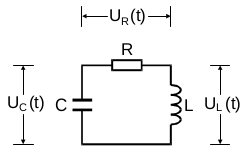
\includegraphics{content/images/V354.png}
  \caption{Gedämpfter L-R-C-Schwingkreis.}
  \label{fig:schwingkreis}
\end{figure}

Für den Stromkreis in Abbildung \ref{fig:schwingkreis} gilt die
DGL:
\begin{equation}
  U_C(t)+U_R(t)+U_L(t)=0
\end{equation}
Für den beschriebenen Strompuls kann die Lösung der DGL mathematisch durch die Überlagerung einer
einhüllenden Funktion und einer sinus/cosinus Funktion dargestellt werden.

\begin{figure}[H]
  \centering
  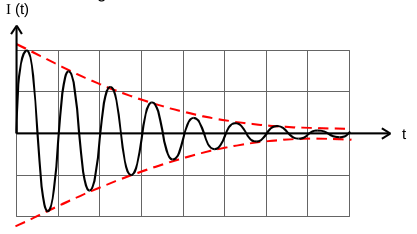
\includegraphics{content/images/dia.png}
  \caption{Dämpfungskurve des Stroms.}
  \label{fig:daempfung}
\end{figure}


\begin{align}
  \symbf{I} &= I_0 e^{-2\pi\mu t}
  \cdot\text{cos}\left(2\pi\nu t+\eta\right)\\
  \symbf{I}_\text{einhüllend} &= I_0 e^{-2\pi\mu t}
  \label{eqn:einhuellend}
\end{align}

\subsection{Grenzwiderstand für den aperiodischen Grenzfall}

\begin{figure}[H]
  \centering
  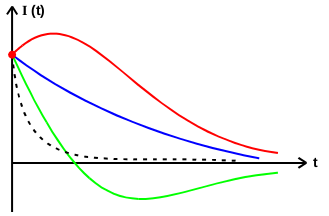
\includegraphics{content/images/dia2.png}
  \caption{Dämpfungskurve des Stroms.}
  \label{fig:aperiodisch}
\end{figure}

Nach der Bestimmung des Dämpfungsverhaltens eines Schwingkreises
wird nun der Widerstand $R_\text{ap}$ berechnet für welchen der
Strom im Schwingkreis am schnellsten gegen null läuft. Dieses
Phänomen wird aperiodischer Grenzfall genannt und wird durch
die gestrichelte Linie in Abbildung \ref{fig:aperiodisch}
dargestellt. Ist der Widerstand zu hoch, so wirkt die Gegeninduktion der
Spule verlangsament und der Graph fällt wie wie der rote oder der
blaue Graph in Abbildung \ref{fig:aperiodisch}, ist er zu hoch
ergibt sich einen Überschwingen wie beim grünen Graphen.
Mathematisch lässt sich dies über die Periodendauer T des
Schwingkreises bestimmen.
\begin{equation}
  T = \frac{2\pi}{\sqrt{1/LC-R^2/4L^2}}
\end{equation}
Der Grenzfall tritt für $T\to\infty$ auf:
\begin{align}
  \implies \frac{1}{LC}&=\frac{R_\text{ap}^2}{4L^2}\\
  \iff R_\text{ap} &=\sqrt{\frac{4L}{C}}
\end{align}

\subsection{Frequenzabhängigkeit der Kondensatorspannung}

\begin{figure}[H]
  \centering
  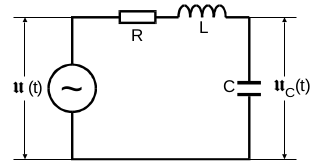
\includegraphics{content/images/kreis2.png}
  \caption{angeregter Schwingkreis.}
  \label{fig:kreis2}
\end{figure}

Für die folgenden Versuchsteile wird ein gekoppelter Schwingkreis
wie in Abbildung \ref{fig:kreis2} verwendet. Die DGL lautet nun:
\begin{equation}
  U_C(t)+U_R(t)+U_L(t)=U_0e^{i\omega t}
  \label{eqn:kreis3}
\end{equation}
Die Eigenfrequenz $\omega_0$ dieses Kreises beträgt:
\begin{equation}
  \omega_0=\frac{1}{\sqrt{LC}}
  \label{eqn:eigen}
\end{equation}
Zunächst wird die Abhängigkeit
der Kondensatorspannung $U_C$ von der Frequenz $\omega$ berechnet.
zu diesem Zweck wird eine Güte q berechnet:
\begin{equation}
  q_\text{exp}=\frac{U_c}{U_\text{erreger}}
  \label{eqn:qexp}
\end{equation}
Diese wird verglichen mit der theoretischen Güteziffer welche sich durch die physikalischen
Eigenschaften des Schwingkreises, sprich $L$, $R$ und $C$, berechnen lässt:
\begin{equation}
  q_\text{theo}=\frac{1}{R}\sqrt{\frac{L}{C}}
    \label{eqn:qtheo}
\end{equation}
Trägt man $U_C$ gegen $\omega$ auf erhält man eine Glockenkurve deren Breite errechnet wird durch:
\begin{equation}
  \omega_+-\omega_-=\frac{R}{L}
  \label{eqn:breite}
\end{equation}

\subsection{Frequenzabhängigkeit der Phase}
Des weiteren lässt sich eine Phase $\phi$ zwischen der Erregerspannung
$U_\text{erreger}$ und der Kondensatorspannung $U_\text{kondensator}$  feststellen und über
die Lösung der DGL \eqref{eqn:kreis3} unter Berücksichtigung der komplexen Impendanz Z berechnen nach:
\begin{equation}
  \phi = \text{arctan}\left(\frac{-\omega RC}{1-LC\omega^2}\right)
  \label{eqn:phase}
\end{equation}
